\section{Technical fundamentals}

This section will explain the technical fundamentals which are necessary to understand the full bachelor thesis.

\subsection{The Scapy library}
\label{sec:scapy}

%UDS stack
\begin{wrapfigure}{r}{0.15\textwidth}
    %
\includegraphics[width=0.1\textwidth]{scapy_logo}
    \raisebox{0pt}[\dimexpr\height-1.5\baselineskip\relax]{
\includegraphics[width=0.15\textwidth]{scapy_logo}}
    %\label{fig:scapy-logo}
\end{wrapfigure}

Scapy is a powerful interactive packet manipulation program. It is able to forge or decode packets of a wide number of protocols, send them on the wire, capture them, match requests and replies, and much more \cite{scapy}.

It is used through a text-based user interface. This has the advantage of being lightweight, and working via ssh connections out-of-the-box. While being mainly a program, it can also be used as a library by importing the necessary classes and interfaces into the own Python program. Scapy supports Python 3 and additionally Python 2, even though its support has ended on 1st of January 2020. The following quote from a maintainer explains the reason behind that \cite{scapy-py2}:

\begin{displayquote}
    Scapy is a tool that can be used in a very large number of situations. Often, you don't get to choose the Python interpreter you have when you run Scapy. So, [...] we need to keep supporting Python 2.7 as long as we can.
\end{displayquote}

One of the core classes in Scapy is the \textbf{Packet} class. All definitions of network packet layers, such as Ethernet, IP, TCP, CAN, UDS and so on, are defined in a class inheriting from that class.

The well-known and simple UDP protocol \cite{rfc768} serves as an illustrative example of how to translate data field specifications (see \autoref{fig:uds_header} for UDP) into a Scapy definition.

%UDP header
\begin{figure}[h]
    \centering
    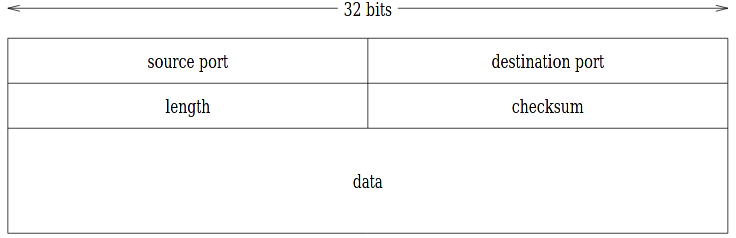
\includegraphics[width=0.7\textwidth]{udp_header}
    \caption{UDP header format \cite{udp_header}}
    \label{fig:uds_header}
\end{figure}

The UDP header format contains four header fields the payload. The header fields are translated literally into the Scapy class \textbf{UDP}. The data field is not part of it because Scapy uses an explicit operator to append data to the header information. This is shown later.

The following code snippet shows the mentioned class in the Scapy library.

\begin{samepage}
\begin{minted}{python}
class UDP(Packet):
   fields_desc = [ShortEnumField('sport', 53, UDP_SERVICES),
                  ShortEnumField('dport', 53, UDP_SERVICES),
                  ShortField('len', None),
                  XShortField('chksum', None)]
\end{minted}
\end{samepage}

As in common programmer language, \textbf{short} specifies 16 bits. Since the UDP header only contains 16 bits fields, the Scapy definition only includes \textbf{short} fields. The first parameter of a field is always the name of this field. \textbf{sport} stands for source port, and \textbf{dport} for destination port.
The next parameter sets the default value for this field. This is defined by the Scapy programmers to the best of their knowledge and not by the official UDP standard. \textbf{53} specifies the DNS protocol.
\textbf{EnumField}s also contain a third argument, a simple dictionary mapping from machine-readable values to human-readable texts. For example, part of the \textbf{UDP\_SERVICES} dictionary is: \mintinline{python}{{53: 'domain', 80: 'www_http'}}.
The difference between the ShortField and XShortField is only the representation, being displayed as a decimal hex and a hex value, respectively.

The following snippet shows some examples of how to instantiate an object of the UDP class and also demonstrates how to append data to the headers with the “/” operator.

\begin{samepage}
\begin{minted}{python}
packet = UDP(dport=80) # is equivalent to:
packet = UDP(dport='www_http')

# Append 0x00 as data
packet = UDP(dport=80) / Raw(b'\x00')
\end{minted}
\end{samepage}

Scapy provides many kinds of sockets to transmit and receive packets. For example the \textbf{L2Socket} and the \textbf{L3PacketSocket}. The difference is that L2Sockets expect a packet containing all information starting from Ethernet (layer 2), while L3PacketSockets expect a packet only containing all information starting from IP (layer 3). The following code snippet illustrates how an Ethernet packet is sent via a L2Socket (Note: Root privileges might be necessary for this to work):

\begin{samepage}
\begin{minted}{python}
# import necessary classes
from scapy.arch.linux import L2Socket
# Create a layer 2 socket specifying the interface name
socket = L2Socket('eth0')
# Create a packet covering layer 2 to 7, targeting the Google server
# This packet starts a TCP handshake, thus the SYN flag is exclusively set
# Set destination port to HTTP and a high source port
packet = Ether() / IP(dst='142.250.185.163') / TCP(flags='S', dport=80, sport=60123)
# sr1 stands for: send receive one
# it sends the given packet and returns the response
response = socket.sr1(packet)
# This displays the response in a human-friendly form
response.show()
\end{minted}
\end{samepage}

The \emph{show} method gives the following output. It has been slightly edited to be more compact and some information has been replaced by placeholders for privacy reasons.

\begin{samepage}
\begin{minted}{text}
###[ Ethernet ]### 
  dst       = 12:34:45:67:89:ab
  src       = 13:37:42:be:ef:00
  type      = IPv4
###[ IP ]### 
     version   = 4
     src       = 142.250.185.163
     dst       = 123.123.123.123
###[ TCP ]### 
        sport     = www_http
        dport     = 60123
        flags     = SA
\end{minted}
\end{samepage}

The SYN and ACK flags are now set as expected for the TCP handshake. Furthermore, the sport of the request is the dport of the response.


\subsection{The CAN bus}

All communication performed and recorded in this paper with an ECU is done via the Control Area Network bus (CAN).

\subsubsection{Basic information}

 Its specification is released in the ISO 11898. Each packet on this bus can transmit up to 8 bytes of payload and has an identifier which a length of either 11 or 29-bits, the former being more common. An identifier does not necessarily have to designate a physical device; it can also indicate one of several modules of a device.
 The maximum data rate is 1 Mbit/sec with a network length below 40 m. The higher the length, the lower the possible data rate, as can be seen in \autoref{tab:can-speed}.

\begin{table}[h]
    \centering
    \begin{tabular}{ccc}
    \hline
    \textbf{Bus Length (m)} & \textbf{Signaling Rate (Mbps)}\\
    \hline
    40 & 1 \\
    100 & 0.5 \\
    200 & 0.25 \\
    500 & 0.10 \\
    1000 & 0.05 \\
    \hline
\end{tabular}
\caption{Suggested Cable Length vs Signaling Rate \cite{slla270}.}
\label{tab:can-speed}
\end{table}

\subsubsection{Advantages}

This bus is robust because it is half-duplex, but still using two wires for the communication with differential signals. This means that if one wire is driven high, the other one is driven low. Thus, the receiver can reliably detect interferences by comparing these signals.

Moreover, CAN busses are using the bus network topology (see \autoref{fig:with-without-can}). This results in a smaller number of wires compared to star topologies, resulting in lower weight, which is an important factor for manufacturers.

%with-without-can
\begin{figure}[h]
    \centering
    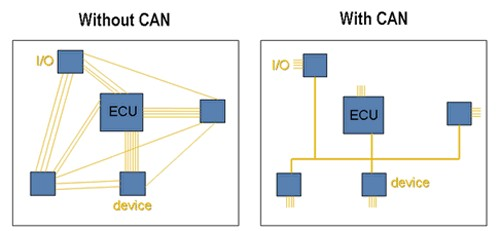
\includegraphics[width=0.7\textwidth]{with-without-can}
    \caption{CAN effect on decreasing the wire quantity \cite{Sharma2016}.}
    \label{fig:with-without-can}
\end{figure}

Last but not least, an important feature for the automotive application domain is the priority support. The lower the identifier, the higher the priority. Hence, if ECU1 and ECU2 transmit a CAN packet at exactly the same time, the packet with the lower identifier wins, the other one is discarded and will be retransmitted. This is called the Carrier Sense Multiple Access with Collision Detection (CSMA/CD) protocol \cite{Sharma2016}. For this reason, diagnostic CAN identifiers tend to have a high identifier \cite{Herrewegen2018}.

\subsubsection{Security vulnerabilities}

Thinking this one step further, CAN is vulnerable to denial of service attacks. This attack can be performed by flooding the CAN bus with zero-identifier messages resulting in drops of legitimate packets \cite{Buttigieg2017}.

Furthermore, Buttigieg et al. \cite{Buttigieg2017} describe three more security issues of the CAN bus protocol in their paper {Security Issues in Controller Area Networks in Automobiles}.
First, CAN packets do not contain any authentication information. An ECU receiving a message is not able to distinguish between a message from a legitimate ECU and a malicious one \cite{Buttigieg2017}. So, for example, if the state of an ECU is changed to a higher privileged state, all devices, including malicious ones, will have access to its newly unlocked services and information. Countermeasures exist in the form of performing authentication, but there is no satisfying solution yet, which fulfills cost-effectiveness, backward compatibility, support for vehicle repair and maintenance, sufficient implementation details, and acceptable overhead \cite{Bozdal2020}.
Also, originally, CAN bus networks lacked network segmentation, since each message is broadcasted and received by each node of the network \cite{Buttigieg2017}. Nowadays, car networks of higher-class cars like Audi and BMW are usually divided into less and more critical segments by so-called Gateway ECUs \cite{Bozdal2020}. Despite the increase in the level of security, this makes it more difficult to maintain the system, which is associated with increased costs \cite{Bozdal2020}.
The final security vulnerability is the lack of data encryption \cite{Buttigieg2017}. Lightweight encryption systems could be implemented, but are limited by the short length of the data field (8 bytes) and the limited computing power of ECUs \cite{Bozdal2020}.

Since all countermeasures described in the previous paragraph are limited, Intrusion Detection Systems (IDS) are emerging, with the advantages of not having to change the current CAN controller and not increasing bus traffic \cite{Bozdal2020}. Such a system has been implemented in the context of the PetS3 project \cite{spahn2018}.

\subsubsection{How to work with the CAN bus}

Virtual CAN interfaces can be used for simulations or simple tests. They are supported natively by Linux without additional actions.
To create a virtual CAN interface, only one command in a Linux shell is required:
\begin{minted}{text}
sudo ip link add vcan0 type vcan
\end{minted}

The most common tool set to work with the CAN bus are the can-utils \cite{can-utils}, which can be usually installed with the package manager of the distributions. For example, the following command displays all messages of the CAN bus on interface \emph{vcan0}:
\begin{minted}{text}
candump vcan0
\end{minted}

Another important task is to send packets. This command sends a CAN packet with the identifier 0x123 and the payload \emph{01 02}:
\begin{minted}{text}
cansend vcan0 123#01.02
\end{minted}

Alternatively, Scapy can be used. There are two implementations of CAN sockets, namely a native one, which uses the native Linux kernel module, and a software-based one, which uses the Python-CAN package. The native implementation only supports Linux but is the preferred one because it uses the POSIX socket API from Linux and brings all its advantages, such as waiting for answers asynchronously without busy-waiting. However, Python-CAN has the advantage of also working on Windows and macOS.

An equivalent Scapy script which accomplishes the same as the just described \mintinline{text}{cansend} command, is:

\begin{samepage}
\begin{minted}{python}
from scapy.contrib.cansocket_native import CANSocket
from scapy.layers.can import CAN
socket = CANSocket("vcan0")
socket.send(CAN(identifier=0x123, data=b"\x01\x02"))
\end{minted}
\end{samepage}

\subsection{The ISO-TP transport protocol for CAN}

CAN packets have a payload size of 8 bytes. This is sufficient for most UDS requests, but not for many UDS responses. Thus, ISO-TP is used as the transport protocol on the CAN bus for UDS communication.

\subsubsection{Basic information}

It is defined in ISO 15765-2 and increases the payload size from 8 bytes to 4095 bytes per message. At least one byte of each CAN packet is then transport protocol information, indicating whether this packet is a single frame or if it only contains a fragment of the actual payload.

\subsubsection{How to work with the ISO-TP protocol}

The can-utils tools also contain applications to handle ISO-TP communication. Since this is never used in this work, but the Scapy implementation is, only the Scapy implementation is explained.

As for the CAN implementation, there are two ISO-TP socket implementations in Scapy. A software and a native implementation. Until including Linux kernel 5.9, the corresponding ISO-TP module for Linux had to be installed separately \cite{isotp-module}. Since Linux kernel 5.10, it is part of the Linux mainline kernel \cite{isotp-commit}. Both implementations handle the ISO-TP metadata themselves, i.e.  fragmentation, defragmentation, etc.

An ISO-TP socket contains a source and destination identifier. They offer the same functionality as the ports for TCP or UDP. The source identifier is the identifier of outgoing CAN packets, and the destination identifier is the identifier expected for incoming packets.

The usage of the native implementation is illustrated in the following code snippet:

\begin{samepage}
\begin{minted}{python}
from scapy.contrib.isotp import ISOTPNativeSocket
socket = ISOTPNativeSocket('vcan0', sid=0x123, did=0x456)
packet = Raw(b'\x01\x02')
socket.send(packet)
\end{minted}
\end{samepage}

\subsection{The UDS protocol}

\subsubsection{Basic information}

UDS stands for \emph{Unified diagnostic services} and is an application protocol defined in ISO 14229. This protocol defines the structures of request and response packets for diagnostic purposes sent over an arbitrary data link \cite{iso14229}.

%UDS stack
\begin{figure}[h]
    \centering
    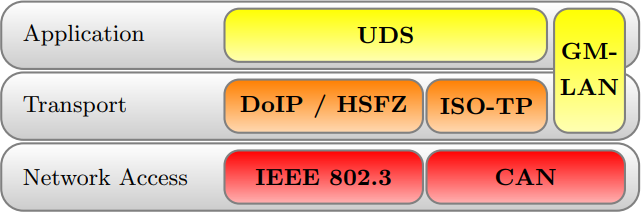
\includegraphics[width=0.7\textwidth]{uds-stack}
    \caption{The most common protocol stack for UDS \cite{Weiss2020}.}
    \label{fig:uds-stack}
\end{figure}

As shown in \autoref{fig:uds-stack}, the most common data links for the UDS protocol are the Ethernet and the CAN bus. Others can and are used as well, explicitly stated in the UDS standard are FlexRay, K-Line and LIN.

\subsubsection{Services}

The UDS protocol defines various services with different purposes.

The DiagnosticSessionControl (DSC) service with the identifier 0x10 is used to enable different diagnostic states in the ECU. All packets requesting this service specify this value as the first byte. The identifiers in the responses are defined as 0x40 added to the request identifier. Thus, for the DSC service the identifier of positive responses is 0x10 + 0x40 = 0x50. A negative response always has the identifier 0x7f.

Another example is the ReadDataByIdentifier (RDBI) service. Data records in an ECU are stored with an identifier as the key. This service allows to read these values from an external device. Since there may be data stored that should not be readable by everyone, there is another service called SecurityAccess (SA, 0x27) that allows to unlock the ECU for external devices.

The SA service uses the challenge–response authentication, in automotive terminology called seed-key protocol. The ECU sends a randomly generated value (the seed) to the client. Both generate a response (the key) and the client sends its response to the ECU. If the keys match for the received and the generated response, the client is authenticated \cite{Herrewegen2018, iso14229}.

\begin{figure}[h]
    \centering
    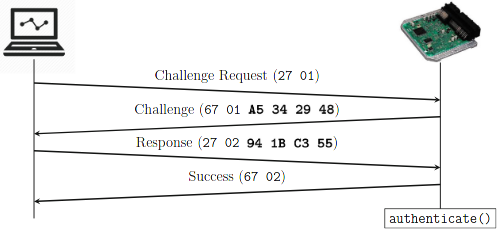
\includegraphics[width=0.7\textwidth]{key-seed}
    \caption{The challenge-response protocol \cite{Herrewegen2018}.}
    \label{fig:key-seed}
\end{figure}


\subsubsection{Implementation of UDS in Scapy}

\begin{samepage}
\begin{minted}{python}
class UDS(ISOTP):
    services = {
         0x10: 'DiagnosticSessionControl',
         # [...]
         0x22: 'ReadDataByIdentifier',
         # [...]
         0x7f: 'NegativeResponse'})
    fields_desc = [
        XByteEnumField('service', 0, services)
    ]
\end{minted}
\end{samepage}

%TODO: Why inherting from ISOTP

The UDS class contains only the service field. Even though the whole UDS protocol is in the application layer, the Scapy implementation starts a new class whenever the subsequent fields depend on one field of the current layer. This is the case here, since the next fields depend on the value of the service field. The service specific fields are defined in their own classes, for example:

\begin{samepage}
\begin{minted}{python}
class UDS_DSC(Packet):
    diagnosticSessionTypes = { ... }
    fields_desc = [
        ByteEnumField('diagnosticSessionType', 0,  diagnosticSessionTypes)
    ]
\end{minted}
\end{samepage}

A UDS packet enabling the extended diagnostic session would be created with:

\begin{samepage}
\begin{minted}{python}
packet = UDS() / UDS_DSC(diagnosticSessionType='extendedDiagnosticSession')
\end{minted}
\end{samepage}

UDS not only allows to read data, but also to write. Which makes it especially critical for security. For example the firmware of an ECU can be updated through this protocol. This usually requires higher privileges, which can be gained through the previously mentioned SecurityAccess service.


\subsection{The UDS Scanner}

The UDS Scanner was implemented in Scapy for the PetS3 project.

\subsubsection{Purpose}

\begin{figure}[h]
    \centering
    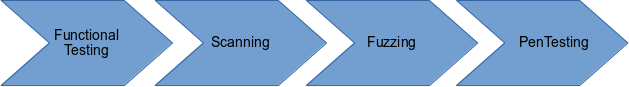
\includegraphics[width=0.8\textwidth]{automotive-security-testing-process}
    \caption{The Automotive Security Testing process.}
    \label{fig:automotive-security-testing-process}
\end{figure}

As \autoref{fig:automotive-security-testing-process} shows, the security testing process in the automotive domain contains a scanning step that aims to detect what services of a protocol are implemented and what information can be retrieved there \cite{Bayer2015}. The UDS Scanner fulfills these tasks. It can also be used for fuzzing and functional testing, even though scanning is its main use-case. The retrieved information assists for the manual PenTesting, the final step in this process.

\subsubsection{Enumerators}

% TODO: Add that it was still work in progress while doing this work
% and thus, that problems occured and had to be fixed.
% Out of scope of this work.

Enumerators are service-specific and create all possible requests for a service.
For example, the enumerator for the DSC service is called UDS\_DSCEnumerator. The most important member of the enumerator classes is the \mintinline{python}{_get_initial_requests} method. The return value is an iterable object which contains all requests for this service. DSC has an eight bit identifier, leading to a maximum of 2\textsuperscript{8} packets for this service. Each enumerator will be executed for each found state of the ECU. So, if an enumerator already ran, and afterwards a new state is found, this enumerator will run again within the same scan with the new-found state.

For a better understanding, the UDS\_DSCEnumerator implementation will be described exemplary.

\begin{samepage}
\begin{minted}{python}
class UDS_DSCEnumerator(UDS_Enumerator, StateGenerator):
    def _get_initial_requests(self, **kwargs):
        session_range = kwargs.pop('session_range', range(2, 0x100))
        return UDS() / UDS_DSC(diagnosticSessionType=session_range)
\end{minted}
\end{samepage}

The method can be given keyword parameters. The only one used here is \mintinline{python}{session_range}. If none is given, which is usually the case, it defaults to the range from 0x02 to 0xff. So, this enumerator creates 254 packets for each state. This service is a StateGenerator, which means its requests can change the state of the ECU. This is detected by the UDS Scanner and the new state will be scanned as well.

So-called staged enumerators contain enumerators where each enumerator is a stage. They start executing the first enumerator for each state, followed by each subsequent enumerator in the same way. For each stage transition (for example $1 \rightarrow 2$ or $2 \rightarrow 3$) connectors can be defined. They are functions with two arguments, containing the previous enumerator and the new enumerator. Here the results of the previous enumerator can be evaluated and the new enumerator can be configured accordingly.

Enumerators can output their results as a text-table. For example:

\begin{samepage}
\begin{minted}{text}
---------------+---------------+---------------+---------------+
               | session1      | session1tp1   | session3tp1   | 
---------------+---------------+---------------+---------------+
TesterPresent: | PR: Supported | PR: Supported | PR: Supported | 
---------------+---------------+---------------+---------------+
\end{minted}
\end{samepage}

This means, the request of the TesterPresent service was positively answered by the ECU in all three found states.

\subsubsection{Procedure}

The UDS Scanner executes all enumerators for each state of an ECU. Enumerators can find new states. So as long as new states are found during an iteration, the scan continues. The default state, i.e. for the currently switched on ECU, is called session1. After each iteration, the ECU is reset to return to the default state. From there, the state to be scanned is activated. An ECU reset is usually done by turning off the ECU, waiting for a few seconds, and turning it on again, although there is an ECUReset service in the UDS protocol. However, the service specification states that the behavior of the ECUReset is implementation-specific, so a power-based reset is the cleaner way.

The following pseudocode aims to make the procedure easier to understand:

\begin{samepage}
\begin{minted}{python}
class UDS_Scanner:
    def scan():
        states = [session1]
        for state in states:
            ecu.reset()
            ecu.enter_state(state)
            for enum in enumerators:
                enum.execute()
        ecu.reset()
\end{minted}
\end{samepage}

